\documentclass{article}  
\usepackage{ijcai15}
\usepackage{times}
\usepackage{cleveref}

\usepackage{amsmath}
\usepackage{amsthm}
\usepackage{graphicx}
\usepackage[font=small,labelfont=bf]{caption}
\DeclareCaptionType{copyrightbox}
\usepackage{subcaption}
\usepackage{amssymb}
\usepackage{amsfonts}
%\usepackage{authblk}
\usepackage{url}
\usepackage{color}
\usepackage[lined, boxed]{algorithm2e}
\usepackage{colortbl}
\definecolor{Gray}{gray}{0.85}

\newcommand{\er}{Erd\H{o}s-R\'{e}nyi } 
\newtheorem{thm}{Theorem}
\newtheorem{cor}{Corollary}
\newtheorem{defn}{Definition}
\newtheorem{propn}{Proposition}
\newtheorem{obs}{Observation}


\title{\Large Constructing Robust Graphs for Community Detection}

%\thanks{This
%work is sponsored by the Assistant Secretary of Defense for Research \&
%Engineering under Air Force Contract FA8721-05-C-0002.  Opinions,
%interpretations, conclusions and recommendations are those of the authors and
%are not necessarily endorsed by the United States Government.}}

\begin{document}

\author{Submitted for blind review.}

%\author{Jeremy Kun\thanks{University of Illinois at Chicago, MIT Lincoln Laboratory} \and Rajmonda S. Caceres\thanks{MIT Lincoln Laboratory} \and Kevin M. Carter\thanks{MIT Lincoln Laboratory}}

\maketitle

\begin{abstract} 

We present a framework called \emph{Locally Boosted Graph Aggregation} for
aggregating multiple noisy networks into a single network so as to improve the
quality of community detection algorithms on the result. LBGA addresses the
problem of finding a single network that faithfully and robustly represents
multiple noisy, complementary underlying data sources. We define a new random
graph model to model such scenarios in community detection called the
\emph{local stochastic block model} (LSBM), and we exhibit the utility of LBGA
on this synthetic model as well as real data sets. LBGA outperforms existing
network aggregation algorithms when ground truth is available, and it produces
high-quality representations of real networks. We argue that LBGA is generic
and can be adapted to other application domains.

\end{abstract}

\section{Introduction}
Community detection methods in machine learning literature generally assume a
single truthful input graph. However, in practical scenarios the data that
comprise a network come from multiple sources which may be noisy and may
disagree~\cite{Leskovec2008}. For example, in a social network one may
communicate with friends via Instagram and family via Facebook. The best way to
aggregate this information is unclear, and the choice of representation heavily
impacts the performance of subsequent data mining algorithms
\cite{Getoor2005,Caceres2011,Miller2014}.  Though the impact of graph
representation on subsequent analysis has been studied, few techniques exist
for learning conducive graph representations. Aggregation is often ad-hoc in
practice, making it difficult to compare algorithms within the same domain
using different data sources.

In this paper, we study the problem of constructing a single graph
representation that accurately reflects the underlying network structure and
allows for better detection of communities scattered across different data
sources. We present an aggregation framework called \emph{Locally Boosted Graph
Aggregation (LBGA)} which simulates an iterative reward system inspired by
boosting and bandit learning. LBGA evaluates the quality of edges locally, so
that it can choose aggregations which most accurately represent the local
structure of communities observed in real
networks~\cite{Aggarwal2011,Leskovec2008}. LBGA relies on the pair of a simple
clustering algorithm and a local heuristic quality measure as a proxy for
evaluating the quality of intermediate results. We empirically show that our
algorithm constructs robust aggregated graph representations for community
detection by testing it on synthetic and real-world data sets and comparing it
to existing aggregation algorithms. 

We emphasize that while this paper specifically addresses community detection,
the edge reward mechanism and the graph aggregation steps
of LBGA are application agnostic. LBGA can be repurposed for graph aggregation
with respect to other applications, a direction we leave for future work. The
paper is organized as follows.  In Section~\ref{sec:related} we review related
literature. In Section~\ref{sec:lbga} we discuss in detail the LBGA framework.
In Section~\ref{sec:experiments} we present the experimental analysis and
results, and Section~\ref{sec:conclusion} we discuss future work.

\section{Related work} 
\label{sec:related}
\subsection{Graph representation learning and clustering}
Our work generally falls under representation learning for graphs, which
includes modeling decisions about the nodes and edges of the graph. Rossi et
al.~\cite{Rossi2012} taxonomize this field, and show that transformations to
heterogeneous graphs can improve the quality of a learning algorithm. Within
their taxonomy our work falls under link re-weighting, which includes the work
of~\cite{Xiang2010,Gilbert2009}. Our setting deviates from these works by 
allowing different edge types between the same pair of vertices. Also, our
approach is stochastic, which we find necessary for learning a robust
representation. 

\cite{Wang14} develops a cross-diffusion based fusion framework called SNF.
Both SNF and LBGA emphasize local similarities versus global ones. SNF's
framework of iterative re-weighting of edges based on message-passing is
similar to LBGA. The LBGA framework is different because the re-weighting is
based on techniques from boosting, and unlike SNF our algorithm does not rely
on consistency across the input graphs. In Section~\ref{sec:comparison} we
demonstrate empirically how LBGA outperforms SNF on all of our synthetic data
sets.
 
Clustering in multilayer
networks~\cite{Papalexakis2013,Tang2009,Tang2012,Mucha2010,Berlingerio2011,kolda2009,Shiga12}
also has close connections to our work. However, the literature does not
address scenarios where the information provided by the different sources is
complementary or the overlap is scarce. Our approach iteratively selects those
edge sources that lead to better clustering quality, independently of
disagreement across the different features. Also, these approaches differ
fundamentally from LBGA in that they do not produce a graph, which could be
used for other purposes. As an example of multi-edge clustering algorithms, we
consider the GraphFuse algorithm~\cite{Papalexakis2013} that falls under the
category of tensor-based clustering. GraphFuse computes the clustering based on
the CP decomposition of the tensor formed by appending the adjacency matrices
of the different graph sources. In Section~\ref{sec:comparison} we demonstrate
that LBGA out-performs GraphFuse in terms of recovering the ground truth
clustering across different datasets considered.

\cite{Rocklin2013,Cai2005} present approaches for identifying the right graph
aggregation, given a complete ground truth clustering or a portion of it. Our
framework requires no such knowledge, but we do use ground truth to validate
our experiments on synthetic data (Section \ref{sec:validation}).

\subsection{Boosting and bandits}
Our framework departs from previous work primarily through its algorithmic
inspirations, namely boosting~\cite{Schapire90} and bandit
learning~\cite{Bubeck12}. In boosting, one assumes the existence of a {\em weak
classifier} whose performance is slightly better than random. In a landmark
paper \cite{Schapire90}, Schapire showed how to combine weak classifiers into a
PAC-learner by a majority voting scheme. One can consider different graph data
sources as weak learners, and ask whether one can ``boost'' them to a good
graph. Unfortunately, our problem setting does not allow pure boosting because
boosting requires access to ground truth labels. Even with reliable input, the
community detection has no single accepted measure of quality. 

In bandit learning an algorithm receives rewards as it explores a set of
actions, and the goal is to minimize a notion of regret. The basic model has
many variants, but two central ones are expert advice and adversaries. Experts
are functions suggesting what action to take in each round, and regret is
measured with respect to the best expert. The adversarial setting involves an
omniscient adversary who sets the experts and rewards so as to maximize regret.
We can imagine graphs as adversarial experts, and adapt bandit learning
techniques to compensate. Indeed, LBGA is a reward system based on the given
application and uses update techniques from bandit learning to learn a graph
representation. In our setting we only care if the aggregate graph is good at
the end, while bandit learning often seeks to maximize cumulative rewards
during learning. There are bandit settings that only care about the final
result~\cite{Bubeck09}, but to the best of our knowledge they do not apply to
our problem. 

The primary technique we use is the Multiplicative Weights Update Algorithm
(MWUA). See~\cite{Arora12} for an overview and an extensive list of successful
applications. The algorithm maintains a weight for each element $x_j$ of a
finite set $X$. In rounds, an element $x_i$ is chosen by sampling
proportionally to the weights, a reward $q_{t,i}$ is received, and the weight
for $x_i$ is multiplied or divided by $(1 + \varepsilon q_{t,i})$, for some
parameter $\varepsilon >0$. After many rounds, the elements with the highest
weight are deemed the best and used for whatever purpose needed. Next, we
describe how this algorithm is adapted to graph aggregation. 

\section{The Locally Boosted Graph Aggregation framework}
\label{sec:lbga}

LBGA can succinctly be described as running multiplicative weights for each
edge, forming a candidate graph representation $G_t$ in each round by sampling
edges, and computing local rewards on $G_t$ to update the weights for the next
round. When $G_t$ converges we produce it as output. The remainder of this
section expands the details of this sketch and our specific algorithm
implementing it. 

\subsection{Framework details}
\label{sec:framework}

Let $H_1, \dots, H_m$ be a set of unweighted, undirected graphs defined on the
same vertex set $V$. We think of each $H_i$ as ``expert advice'' suggesting for
a pair of vertices $u,v \in V$ whether to include edge $(u,v)$ or not. Our
algorithm combines the $H_i$ into a single graph $G^*$ suitable for the
proposed application. We present LBGA in the context of community detection,
noting generalizations. Each round has four parts: producing the aggregate
candidate graph $G_t$, computing a clustering $A(G_t)$ for use in measuring the
quality of $G_t$, computing the local quality of each edge, and updating the
weights for the edges. After $T$ rounds we output $G^* = G_T$.

\textbf{Aggregated Candidate Graph $G_t$}: In each round construct $G_t$ as
follows. Maintain a weight $w_{u,v,i}$ for each graph $H_i$ and each edge
$(u,v)$ in $H_1 \cup \dots \cup H_m$. Normalize the set of all weights for an
edge $\mathbf{w}_{u,v}$ to a probability distribution over the $H_i$. For each
edge $u,v$, sample an $H_i$ according to this distribution and include the edge
in $G_t$ if it is present in the drawn $H_i$. 

\textbf{Event $A(G_t)$}: After the graph $G_t$ is produced, run a clustering
algorithm $A$ on it to produce a clustering $A(G_t)$. In this paper we fix $A$
to be the Walktrap algorithm~\cite{Walktrap}, though we have observed the
effectiveness of other clustering algorithms as well. In general $A$ can be any
event, and in this case we tie it to the application by making it a simple
clustering algorithm.

\textbf{Local quality measure}: Define a \emph{local quality measure}
$q(G,e,c)$ to be a $[0,1]$-valued function of a graph $G$, an edge $e$ of $G$,
and a clustering $c$ of the vertices of G. The quality of $(u,v)$ in $G_t$ is
the ``reward'' for that edge, and it is used to update the weights of each
input graph $H_i$.  More precisely, the reward for $(u,v)$ in round $t$ is
$q(G_t, (u,v),A(G_t))$.

\textbf{Update Rule}: Update the weights using MWUA as follows. Define two
learning rate parameters $\varepsilon > 0, \nu > 0$, with the former being used
to update edges from $G_t$ that are present in $H_i$ and the latter for edges
not in $H_i$. In particular, suppose $q_{u,v}$ is the quality of the edge
$(u,v)$ in $G_t$. Then, the update rule is defined as follows:
\[
w_{u,v,i}=
\begin{cases}
w_{u,v,i}(1 +\varepsilon q_{u,v}), & \text{if } (u,v) \in H_i \\
w_{u,v,i}(1 - \nu q_{u,v}), & \text{if } (u,v) \not \in H_i .
\end{cases}
\]
 \subsection{Quality measures for community detection}
\label{sec:quality-measures}
We presently describe the quality measure we use for community detection. First
we define {\em edge consistency}, which measures whether an edge has endpoints
in the same cluster or across clusters:
\[
   EC_{u,v}=
   \begin{cases}
   1, & \text{if  }c(u) = c(v) \\
   -1,  & \text{if  }c(u) \neq c(v).
   \end{cases}
\]
We also define \emph{neighborhood overlap} ($NO$), which asserts that vertices
sharing many neighbors are likely to be in the same community. NO declares the
quality of $(u,v)$ to be the (normalized) cardinality of the intersection of
the neighborhoods of $u$ and $v$, namely $NO_{u,v}=\frac{|N(u) \cap
N(v)|}{|N(u) \cap N(v)| + log(|V|)},$ where $N(x)$ is the neighborhood of $x$.
Our quality metric, \emph{consistentNO}, combines edge consistency with
neighborhood overlap by multiplying the two functions. We have also run
experiments using more conventional neighborhood metrics, such as the Dice and
Jaccard indices~\cite{Dice1945}). ConsistentNO outperforms them by
at least 10\% in our experiments and for brevity we omit the results. 

\subsection{LBGA implementation} 
We give pseudocode for our implementation of LBGA in Algorithm~\ref{alg:nef}.
The runtime of LBGA is $O(T(|E| Q(n) + A(n)))$, where $|E|$ is the number of
edges, $Q(n)$ is the runtime of evaluating the quality function, $A(n)$ is the
runtime of evaluating the event $A$, and $T$ is the number of rounds.
Algorithm~\ref{alg:nef} improves this by fixing edges whose weights have grown
$ > 1-\delta$ or $< \delta$ for a new parameter $\delta$. As LBGA learns, the
sampling procedure becomes substantially sublinear in the number of edges.
Penalizing non-edges ($\nu > 0$) also improves runtime, and LBGA is stable to
minor variations in $\varepsilon$ and $\delta$. Moreover, our algorithm
empirically scales linearly with the size of the input.

\begin{algorithm}[tbh]
\caption{Optimized implementation of LBGA. Note that $1_E$ denotes the
characteristic function of the event $E$.}
\label{alg:nef}
   \DontPrintSemicolon
   \SetAlgoLined
   {\footnotesize
   \KwData{Unweighted graphs $H_1, \dots, H_m$ on the same vertex set $V$, a
clustering algorithm $A$, a local quality metric $q$, three parameters
$0 < \varepsilon, \nu, \delta < 1/2$}
   \KwResult{A graph $G$}
   Initialize a vector $\mathbf{w}_{u,v} = \mathbf{1}$ for all $u \neq v \in V$\;
   Let $U$ be the edge set of $H_1 \cup \dots \cup H_m$\;
   Let $G_\textup{learned} = (V, \varnothing)$ \;
   \While{$|U| > 0$}{
      Let $G$ be a copy of $G_{\textup{learned}}$\;

      \For{$(u,v) \in U$}{
         Let $p_{u,v} = \frac{\sum_i w_{u,v,i} 1_{\left \{(u,v) \in H_i \right \}}}{\sum_i w_{u,v,i}}$ \;
         Flip a coin with bias $p_{u,v}$\;
         If heads, include $(u,v)$ in $G$.
      }

      Cluster $G$ using $A$\;

      \For{$(u,v) \in U$}{
         Set $p = q(G, A(G), (u,v))$\;
         \For{$i = 1, \dots, m$}{
            \eIf{$(u,v) \in H_i$}{
               Set $w_{u,v,i} = w_{u,v,i} (1 + \varepsilon p)$\;
            } {
               Set $w_{u,v,i} = w_{u,v,i} (1 - \nu p)$\;
            }
         }

         Let $p_{u,v} = \frac{\sum_i w_{u,v,i} 1_{\left \{(u,v) \in H_i \right \}}}{\sum_i w_{u,v,i}}$ \;
         \If{$p_{u,v} > 1-\delta$}{
            Add $(u,v)$ to $G_{\textup{learned}}$, remove it from $U$\;
         }
         \If{$p_{u,v} < \delta$}{
            Remove $(u,v)$ from $U$\;
         }
      }
   }
   Output $G$\;
}
\end{algorithm}

\section{Experimental analysis}
\label{sec:experiments}
We describe the datasets used for analysis and provide quantitative results for
the performance of Algorithm~\ref{alg:nef}. In all of our experiments LBGA was
run with parameters $\varepsilon=\nu=0.2, \delta=0.05$.

\subsection{Synthetic datasets}
\label{sec:synthetic-model}

Our primary synthetic data model is a generalization of the stochastic block
model of~\cite{Wang87}. We construct a probability distribution $G(n_i, p_i,
r_i)$ over graphs as follows. Given a number $n$ of vertices and a list of
cluster (block) sizes $\mathbf{n}=\{n_1, \dots, n_k\}$ with $n=\sum_i n_i$,
partition the $n$ vertices into $k$ blocks $\{b_1, \dots, b_k\}$ with
$|b_i|=n_i$. Define $k$ graphs $G_1, \dots, G_k$ and set the probability
of an edge occurring in $G_i$ with both endpoints in block $b_i$ to $p_i$, all
others occuring with probability $r_i$. We call this model the \emph{local
stochastic block model} (LSBM). To contrast, we define the \emph{global
stochastic block model} (GSBM) by setting the probability of an edge occuring
in $G_i$ with endpoints in the same block (any block, not just block $b_i$) to
be $p_i$, all others with probability $r_i$. Finally, we include \emph{\er
random graphs}~\cite{Erdos60} alongside LSBM (e.g., LSBM-3) to capture a range
of structure and noise combinations.

\begin{table}
\begin{tabular}{| l | l |}
\hline
Dataset & Parameters\\
\hline 
\hline
LSBM-1  &  $m=k=4, n_i=125, p_i=0.2, r_i=0.05$ \\
LSBM-2  &  $m=k=4, n_i=125, p_i=0.3, r_i=0.05$ \\
LSBM-3  &  $m=5,k=4, n_i=125, p_i=0.3, r_i=0.05$, \\ 
        &  $i = 1, \dots, m, p_5= r_5 = 0.01$ \\
\hline
GSBM-4  &  $m =k= 4, n_i=125, p_1=0.1625, $ \\ 
        &  $p_2 = 0.125, p_3 = 0.125, p_4 = 0.0875, r_i = 0.05$ \\
       
GSBM-5  &  $m=k=4, n_i=125, p_1=0.15, p_2=0.1,$ \\ 
        &  $p_3=p_4=0.05, r_i = 0.05, i=1, \ldots, m$ \\

\hline
ER only &  $m=4, p_i=r_i=0.01$ \\
DBLP    &  $n = 3153, m = 2$ \\
RMining &  $n = 90, m = 6$ \\
Enron   &  $n = 145, m = 2, \alpha=0.9$ \\
\hline
\end{tabular}
\caption{Description of datasets analyzed. Total number of vertices in each
synthetic source graph is $n=500$. The number of graph sources is $m$. The
number of clusters is $k$. The number of vertices in cluster $i$ is $n_i$. 
The within- and across-cluster edge probabilities for graph source $i$ are
$p_i$ and $r_i$, respectively.}
\label{datasets}
\end{table}


\subsection{Real datasets} 
We use a subset of \emph{DBLP}~\cite{Ley02}, an online database of research in
computer science. We take data from two conferences: the Symposium on the
Theory of Computing (STOC), and the Symposium on Foundations of Computer
Science (FOCS). Each of the 3153 nodes represents an author, and we use two
graphs on this vertex set: the {\em co-authorship} graph and the {\em title
similarity} graph. For the latter, we add an edge between two author vertices
if any of their paper titles contain at least three words in common (excluding
stop words), and the weight of this edge is the number of such pairs.

\emph{RealityMining} \cite{RealityMining} was a 9-month experiment in 2004
which tracked a group of 90 individuals at MIT via their cell phones. The
dataset includes voice calls, bluetooth scan events, cell tower usage, and
self-reported friendship and proximity data. We used data between 2004-09-23
19:00:00 and 2005-01-07 18:00:00 (UTC-05:00). Nodes are individuals in the
study, and weighted edges correspond to the total duration of voice calls, the
total amount of time two individuals used the same cell tower, the total number
of bluetooth events, and the results of the friendship/proximity surveys for a
total of 6 graphs. 

Finally, the \emph{Enron} email dataset~\cite{EnronConf} is a corpus of
over 600,000 emails sent between 145 employees of the Enron Corporation in the
early 2000's. We produced two graphs from the Enron data, one for peer-to-peer
email communication and one for topic similarity in the email content. The
vertices are individuals. For email, edges are weighted by the
number of emails sent. We used Mallet~\cite{mallet} to generate the LDA topic
model for the content of Enron email data, aggregating into one document all
the email content sent by each employee. Each document is represented by 60
topics. We measure cosine distance of the topic vectors, and consider an edge
as present if the cosine distance was above a specified threshold value
$\alpha$ discussed in Section~\ref{sec:enron-results}. Table~\ref{datasets}
contains a summary of all the datasets used for the experimental analysis and
their parameters. 


\subsection{Validation procedure} \label{sec:validation}

We now state how we evaluate the quality of LBGA's output.

{\em Recovery of Inherent Clusters.} Since the output of LBGA is a graph, we
use the walktrap clustering algorithm to extract communities for analysis. When
ground truth communities are available we compare them with LBGA's communities
using Normalized Mutual Information~\cite{Danon05}. Otherwise we relate our
clusters to known features of the dataset. 

{\em Quality of Graph Representation.} In addition to producing a good
clustering, an ideal graph representation also removes cross-community edges
and produces a sparser representation. We use the standard Newman modularity
measure~\cite{Newman06} and conductance~\cite{Leskovec2008} to
measure this. Note that \emph{higher} modularity scores and \emph{lower}
conductance scores signify stronger community structure. We note two extreme
graph representation cases, the empty graph which is perfectly modular and the
union graph which is a trivial aggregation. To signal these cases in our
results, we display the \emph{sparsity} of the produced graph $G^*$, i.e. the
fraction of edges in $G^*$ out of the total set of edges in all input graphs. 

{\em Recovery of Graph Source Contribution.} In our experiments some input
graphs contribute more to uncovering the underlying community structure, and
should have higher edge weights on average. As such we display the average
weights of the input graphs, e.g. in Figure~\ref{fig:local-sbm}. 

\subsection{Experimental results}
\label{sec:results}

Table~\ref{table:results} states the numerical results of our experiments. As a
baseline, we computed the modularity and conductance values of the union of the
input graphs with respect to the ground truth (for synthetic) or the Walktrap
clusterings (for the real world). For synthetic examples, we compare our
results with GraphFuse~\cite{Papalexakis2013} and SNF~\cite{Wang14} algorithms.
Overall, LBGA converges to graphs with high modularity and low conductance.
LBGA produces graph representations that induce correct clusterings in almost
all cases where ground truth is known, the challenging case being when the
noise rate is close to known detectability thresholds. 

\subsubsection{Synthetic}
Figure~\ref{fig:local-sbm} depicts a run of Algorithm~\ref{alg:nef} with
consistentNO on the dataset LSBM-3. LBGA converges quickly to a graph with a
perfect clustering and high modularity. We plot the number of edges in $G_t$
over time and the average vertex-pair weight for each input graph. LBGA
produces a graph using with 40\% sparsity and weights edges from the \er source
appropriately. Our algorithm hence achieves a high quality graph while
preserving and highlighting the underlying community structure. 

\Cref{fig:local-sbm,fig:erpvaries} also demonstrate that LBGA does not falsely
boost noise to report community structure where none is present.
Figure~\ref{fig:erpvaries} depicts the behavior of LBGA on a dataset of only
\er random graphs. LBGA produces aggregate graphs whose modularity values are
low and conductance values are high. We see a clear phase transition in
performance around $p = 0.3$ corresponding to the \er graphs becoming
triangle-dense and therefore less distinguishable from graphs that are a single
community. Tolerance to such dense levels of noise is unavoidable. 

\begin{figure}[t]
\begin{centering}
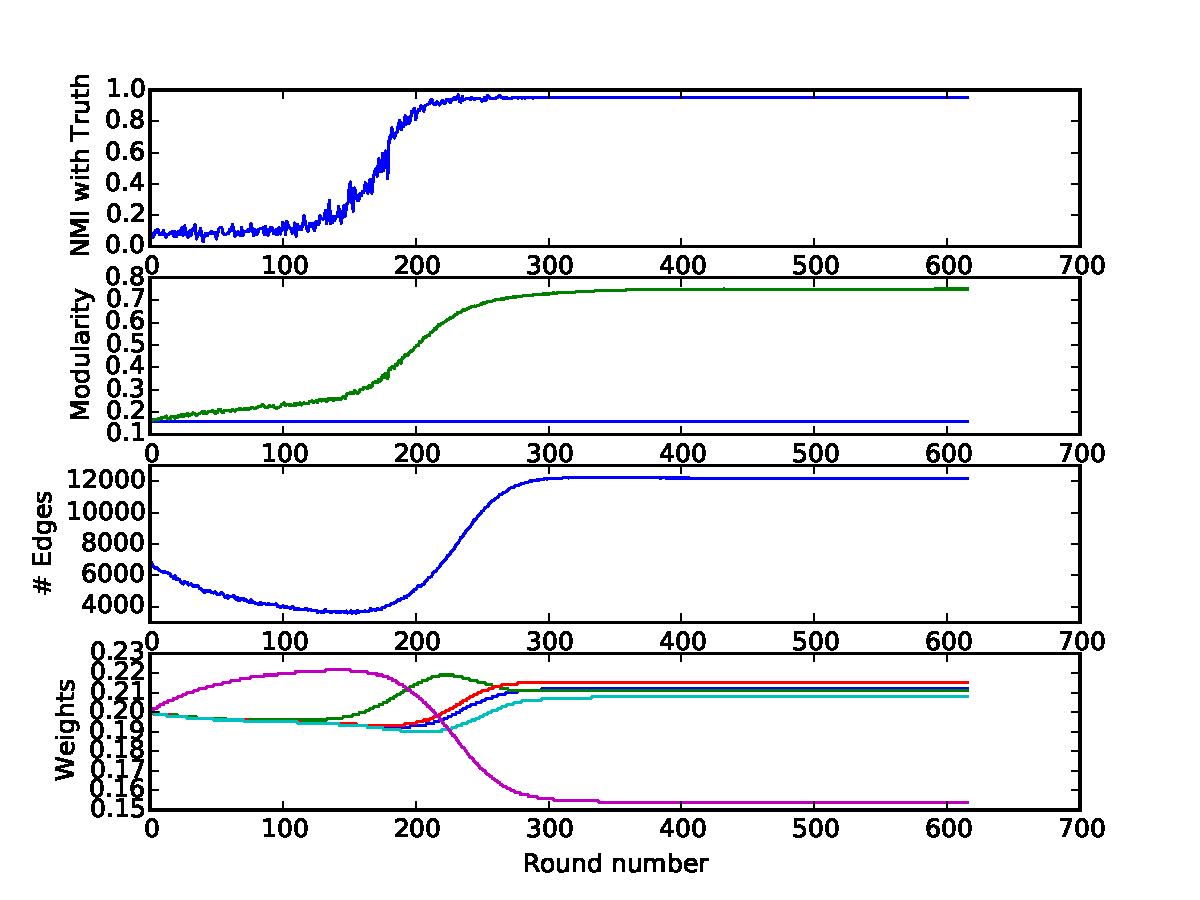
\includegraphics[width=\columnwidth]{figures/LBM-SNR=6+ER-consistentNO+NEF.pdf}
\par\end{centering}
\caption{Graph representation learning for LSBM-3. The LBGA parameters are
$\varepsilon=\nu=0.2, \delta=0.05$. Plots in order top to bottom: 1. NMI of
$A(G_t)$ with the ground truth clustering, 2. modularity of $G_t$ w.r.t.
$A(G_t)$, with the horizontal line showing the modularity of the union of the
input graphs w.r.t. ground truth, 3. the number of edges in $G_t$, 4.  the
average probability weight of vertex pairs for $H_i$.  The \er graph converges
to low weight by round 300, even though it is initially favored. Hence
LBGA can recover from bad luck and does not boost noise.} 
\label{fig:local-sbm} 
\end{figure}

\begin{figure}[t]
\begin{centering}
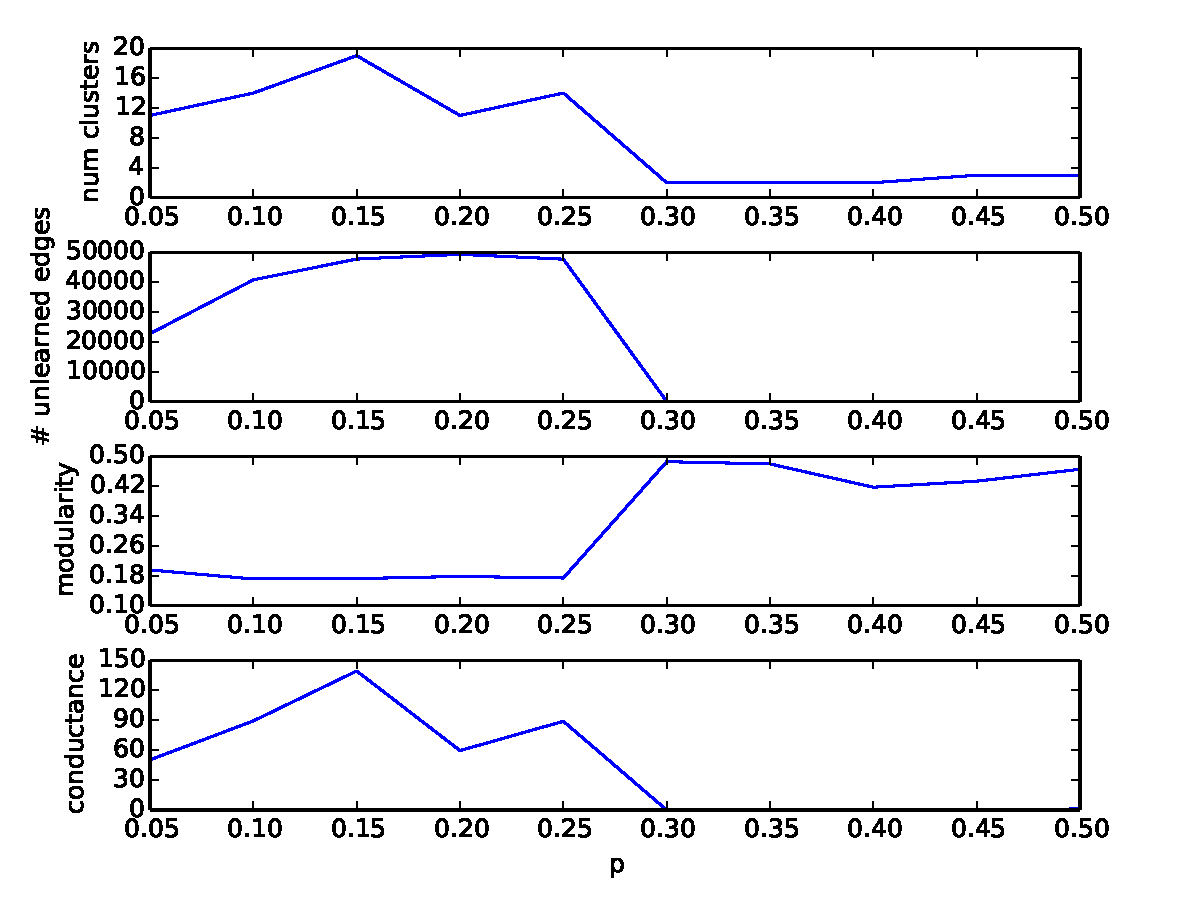
\includegraphics[width=\columnwidth]{figures/er-consistentNO-varying-p.pdf}
\par\end{centering}
\caption{Statistics about the aggregate graph produced by LBGA after 500 rounds
on a suite of 4 \er random graphs on 500 nodes and varying edge probability
$p$.} 
\label{fig:erpvaries}
\end{figure}

\subsubsection{DBLP} 
Table~\ref{table:results} shows LBGA producing an aggregate DBLP graph of
modularity exceeding the baseline and using significantly fewer edges. Our
algorithm selects title similarity as having more influence in recovering
communities for the STOC/FOCS conferences. We also manually inspected the
resulting clusters, they incorporate both membership and coauthorship. For
example, Mikko Koivisto, Thore Husfeldt, Petteri Kaski, and Andreas
Bj\"{o}rklund have coauthored over 15 papers in combinatorial optimization.
They naturally fall within a small coauthorship cluster.  However, title
similarity splits these researchers across two clusters due to differences in
their non-coauthored work. They fall in the same cluster in the aggregate
graph, which includes researchers who are either coauthors with one of the four
or have done much work in the same field. 


\subsubsection{RealityMining \& Enron} \label{sec:enron-results}

For RealityMining, LBGA's output contains two dense clusters corresponding
exactly to the MIT Media Lab and the Sloan Business School, with only three
edges crossing the cut. In addition, this graph uses only 63.5\% of the total
edges available. For Enron, LBGA achieves similar results. In addition,
Figure~\ref{fig:enron-comparison} depicts the output of LBGA, showing a clear
community structure.  The small clusters are lower-level employees, and the big
clusters are managers. Moreover, there was a known fantasy sports club within
the network~\cite{Mccallum05}, and these individuals all fall in a single
cluster of $G^*$. 

The modularity of RealityMining and Enron are smaller with LBGA than the
baseline. We argue that this is caused by small clusters produced by LBGA,
modularity is known to be inaccurate for small clusters~\cite{Fortunato07}.
Indeed, LBGA outperforms the baseline with respect to conductance. 

%Figure~\ref{fig:reality-mining-comparison} shows the favorable structure of the
%RealityMining dataset after being passed through LBGA (and the noisy input
%data), and Figure~\ref{fig:enron-comparison} gives a similar picture for the
%Enron dataset. 

%\begin{figure}[t]
%\begin{centering}
%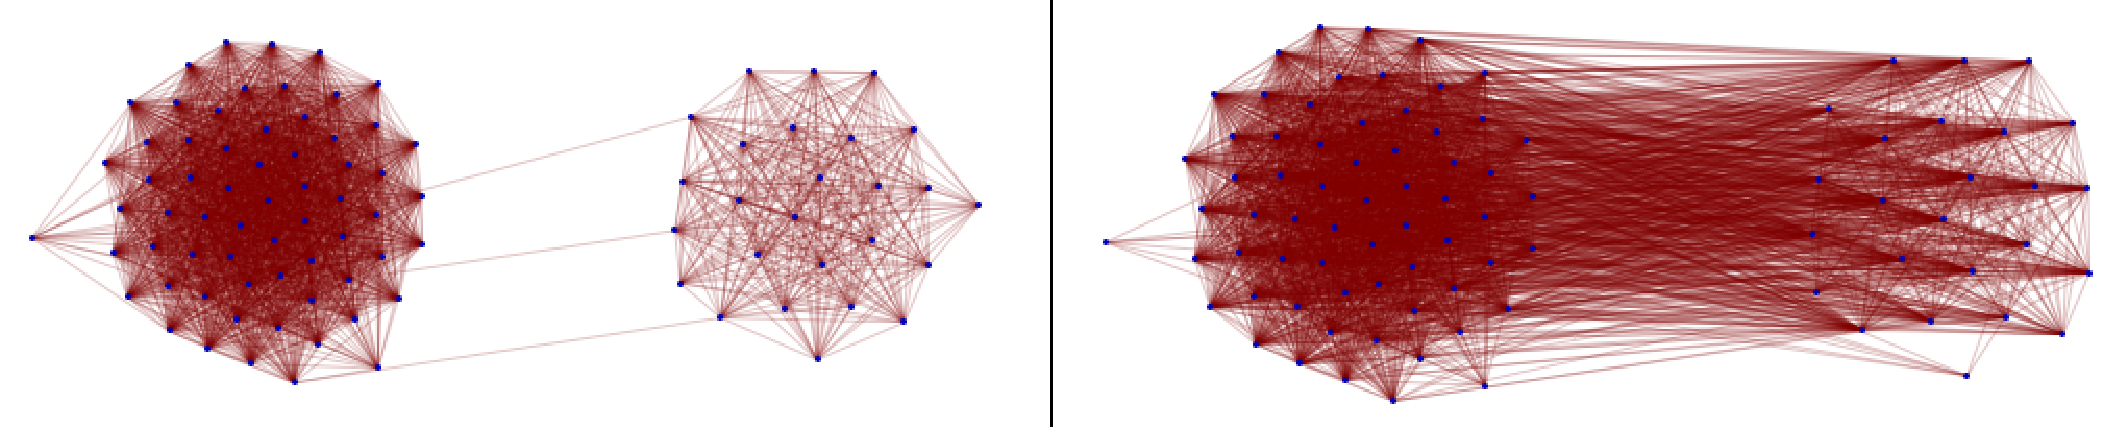
\includegraphics[width=\columnwidth]{figures/reality-mining-comparison.pdf}
%\par\end{centering}
%\caption{Left: the results of LBGA on the RealityMining dataset. Right: the
%input graph of Bluetooth scan events. LBGA was run with $consistentNO$, $\nu =
%\varepsilon = 0.2$, $\delta = 0.05$} 
%\label{fig:reality-mining-comparison}
%\end{figure}

\begin{figure}[t]
\begin{centering}
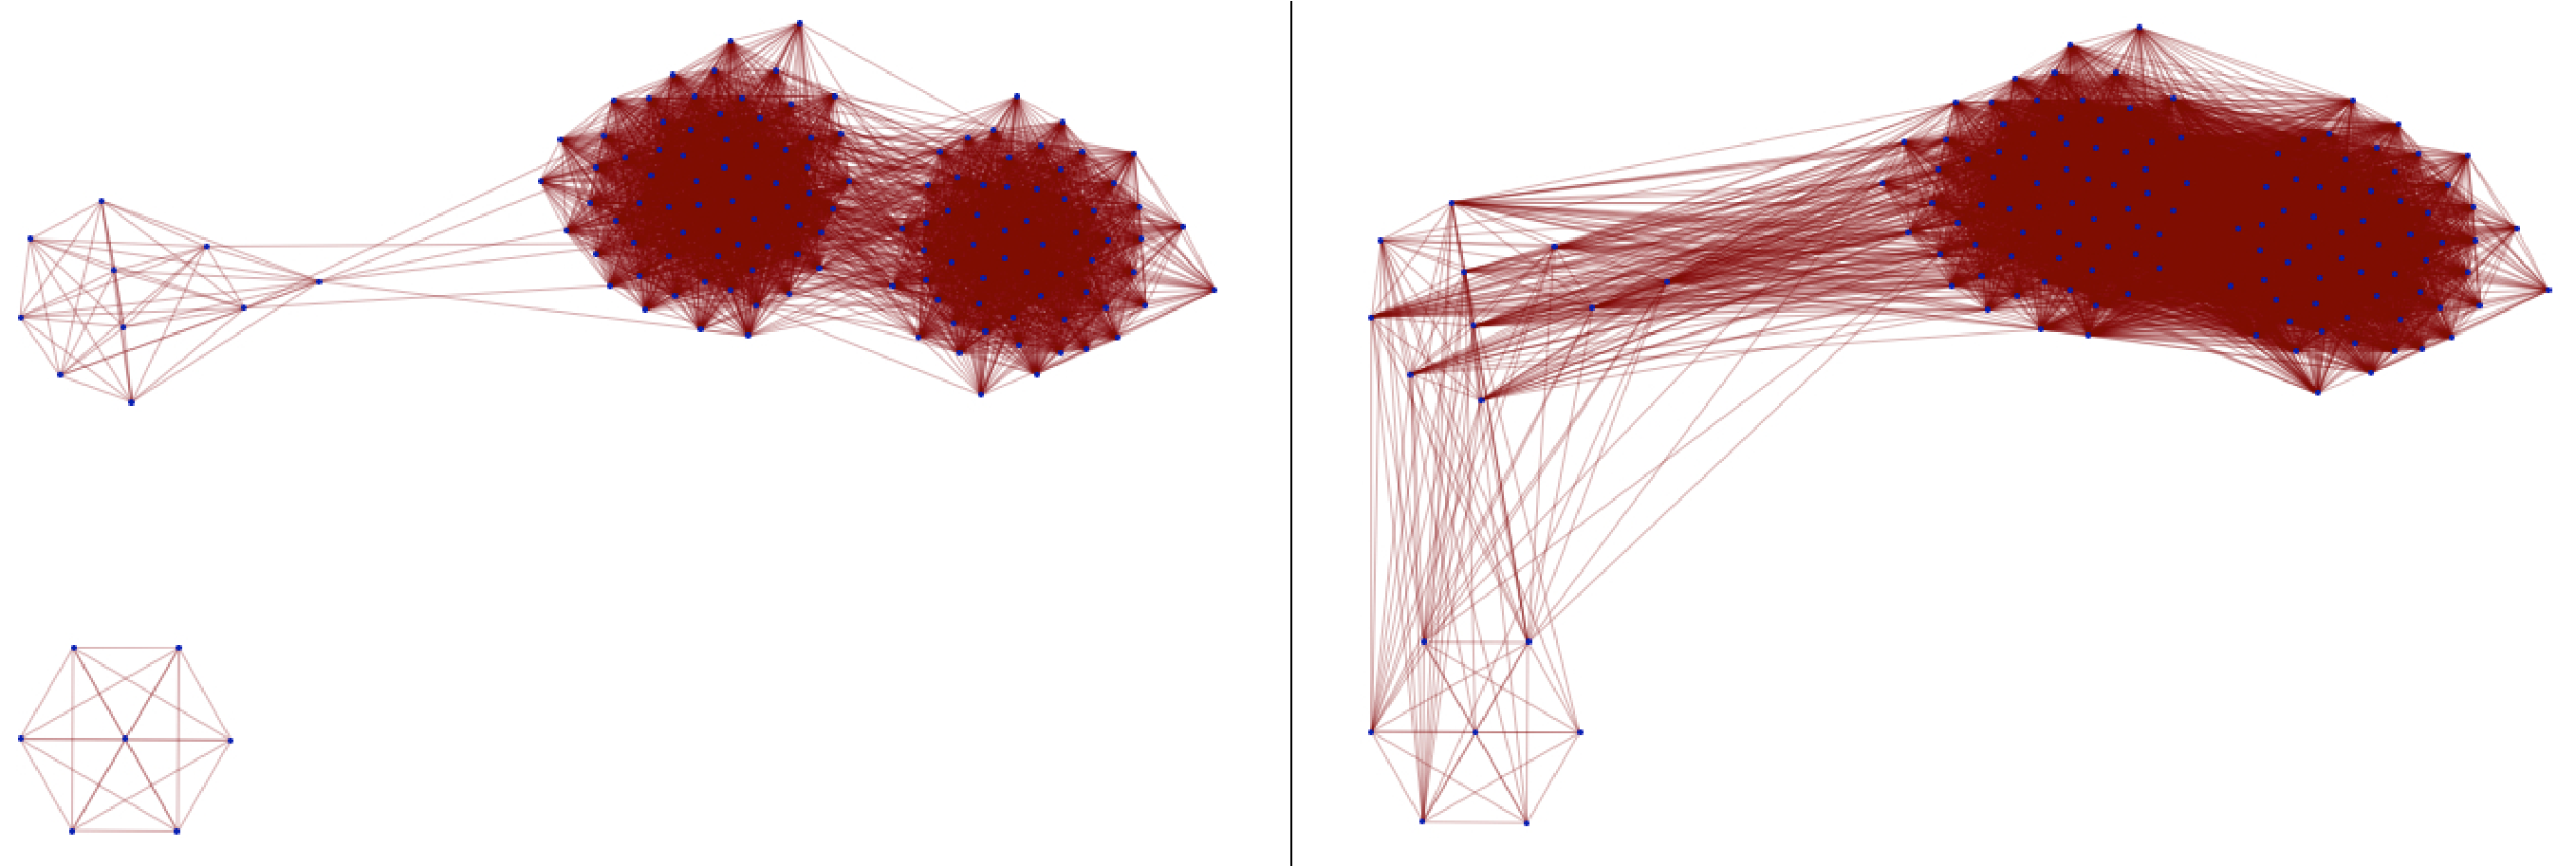
\includegraphics[width=\columnwidth]{figures/enron-comparison.pdf}
\par\end{centering}
\caption{Left: the results of LBGA on the Enron dataset. Right: the input graph
of topics.}
\label{fig:enron-comparison}
\end{figure}


\subsection{Comparison with GraphFuse and SNF}
\label{sec:comparison}
We compare LBGA with GraphFuse~\cite{Papalexakis2013}, a multi-graph clustering
algorithm and SNF~\cite{Wang14}, a graph fusion algorithm. We use NMI with the
ground truth as the performance measure. For the comparison analysis we have
only considered the synthetic datasets where the notion of ground truth is
known. Table~\ref{table:results} contains the comparison results. 

LBGA outperforms SNF in all cases, and by a particularly large margin on the
LSBM model. LBGA also outperforms GraphFuse on both the global block models and the
lower-noise local block models LSBM-2 and LSBM-3. LBGA also produces very
sparse representations that may be useful for future analysis, while GraphFuse
and SNF produce only a clustering.

\begin{table*}
\large
\setlength\extrarowheight{7pt}
\centering
\resizebox{\textwidth}{!}{
\begin{tabular}{| l | c c c | c | c | c c c c |}
\hline 

\multicolumn{1}{| l}{} &  \multicolumn{3}{c|}{Union Graph} & \multicolumn {1}
{c|}{GraphFuse} & \multicolumn {1} {c|}{SNF} & \multicolumn{4}{c|}{LBGA:
ConsistentNO}\\ \hline
Dataset  & Mod. & Cond. & NMI & NMI & NMI & Modularity & Conductance & NMI & Sparsity \\
\hline
\hline

GSBM-4   &  0.178 &  10.678   &  1.000    &  0.716  & 0.658 &  0.739 &  0.084 &  1.000 &  0.433  \\
GSBM-5   &  0.093 &  15.368   &  0.636    &  0.616  & 0.436 & 0.727 &  2.121 &  0.619 &  0.235  \\
\hline
LSBM-1   &  0.103 &  14.725   &  0.724    &  0.686  & 0.099 &  0.679 $\pm$ 0.114 &  9.962 $\pm$ 23.0 &  0.503 $\pm$ 0.05 &  0.263 $\pm$ 0.04 \\
LSBM-2   &  0.166 &  11.233   &  0.992    &  0.760  & 0.180 & 0.740 &  0.084 &  0.992 &  0.420  \\
LSBM-3   &  0.166 &  11.216   &  1.000    &  0.779  & 0.209 &   0.737 &  0.104 &  1.000 &  0.422 \\

\hline
ER only  & -0.002 & 24.729    &  -        & -   &-    &  0.193 & 112.947 & -    &  0.230  \\
\hline
DBLP     & 0.386  & 1368.859  &  -        & -    &-   &  0.695 & 159.286 & -    &  0.632  \\
RMining  & 0.452 & 70.314 &   -      & -   &-    &  0.246 & 0       & -    &  0.646  \\
Enron  & 0.559 & 134.572 &  -   & - & -&  0.444  & 0.594 & -   &  0.631  \\
\hline
\end{tabular}
}
\caption{LBGA performance results, compared to GraphFuse, SMF, and a baseline
union aggregation. All datasets in this table were run with $consistentNO$
using $\varepsilon = \nu = 0.2, \delta = 0.05$. Union modularity and
conductance for real datasets was computed with the walktrap clustering. Values
were averaged over 10 trials, and when variances $\sigma^2 > 10^{-4}$ were
observed, values are reported with $\pm \sigma$.} 
\label{table:results}
\end{table*}

\subsection{Sensitivity analysis} \label{sec:sensitivity-analysis} 

We analyze the sensitivity of LBGA to noise. In
Figure~\ref{fig:sensitivity-analysis} we display NMI for the LSBM model and
varying intra-cluster edge probability $p_i$ and varying signal-to-noise
ratios. As expected, NMI falls as the noise rate $r_i$ increases. LBGA reaches
higher quality and maintains the quality longer for denser graphs, which is
also consistent with our expectations. At a signal to noise ratio of 2 or less,
the NMI drops to non-useful levels regardless of $p_i$. The sharp drop in
quality is related to well-known phase transitions for community
detectability~\cite{nadakuditi2012}.

\begin{figure}[bht]
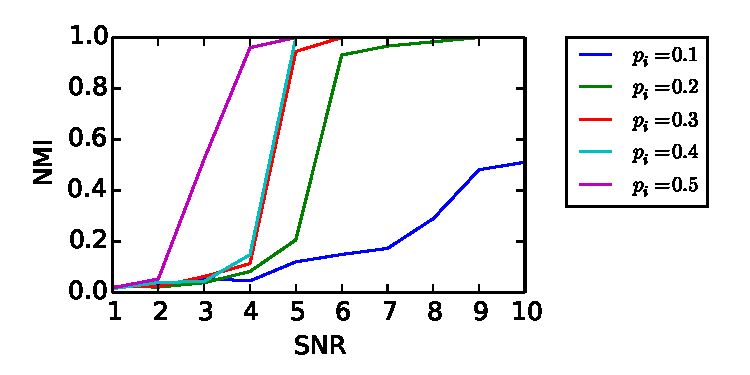
\includegraphics[scale=0.7]{figures/signal-to-noise-consistentNO.pdf}
\caption{Performance of LBGA (measured by NMI) as a function of SNR for the
LSBM model with different probabilities $p_i$ for $consistentNO$.} 
\label{fig:sensitivity-analysis}
\end{figure}

\section{Conclusion}
\label{sec:conclusion}
LBGA offers a flexible, local aggregation method for combining different graph
sources in order to better represent community structure in networks. We derive
LBGA from a solid theoretical foundation in boosting and bandit learning, and
demonstrated LBGA as a proof of concept on synthetic and real networks. LBGA
also simplifies the task of designing a graph aggregation algorithm into
utilizing a principled quality measure $q$ and global event $A$. Doing so
allows us to connect the utility of the graph representation to the application
of interest. 

There are some natural directions to pursue in further studying LBGA. For
community detection, we can improve LBGA in a number of ways. Our consistentNO
metric is simple, and a more sophisticated metric comparing a local
neighborhood to a given null model is likely to provide improvements.
Additionally, we use the walktrap clustering algorithm as a black box in the
``event'' step of LBGA, and walktrap makes some simplifying decisions to arrive
at a final clustering. A direction for future work is to use a modified
walktrap event that outputs raw similarity values before constructing a
clustering, and incorporating this data into the quality measure. Finally,
preliminary results of the authors and others show that LBGA can also be
improved by incorporating a consensus technique using LBGA as a black box, and
that LBGA can detect hierarchical community structure. Further study of these
is needed for a better understanding of LBGA.

Another primary direction is to study the utility of LBGA for other data mining
techniques, such as link prediction. Since LBGA is modular, one can adapt LBGA
to a new application domain simply by defining an event and quality function.

A final direction is to use proof techniques from boosting and bandit learning
to provide strong theoretical guarantees on the performance of LBGA. The
authors have some preliminary results in this direction that have not been
included in this manuscript for brevity.

%\section{Acknowledgements} We thank Vineet Mehta for providing us with the
%Enron topic model data, and for his many helpful discussions.

\bibliographystyle{plain}
\bibliography{lbga}

\end{document}

